
\documentclass[residuals.tex]{subfiles}
\begin{document}
\Large
\newpage
\subsection{\texttt{resid} - Extracting Model Residuals}

% =========================================================%

\begin{itemize}
\item \texttt{residuals} is a generic function which extracts model residuals from objects returned by modeling functions. 

\item The abbreviated form \texttt{resid} is an alias for residuals. It is intended to encourage users to access object components through an accessor function rather than by directly referencing an object slot. 

\item All object classes which are returned by model fitting functions should provide a residuals method. (Note that the method is for \texttt{residuals} and not \texttt{resid}.) 

\item Methods can make use of \texttt{naresid} methods to compensate for the omission of missing values. The default, nls and smooth.spline methods do. 
\end{itemize}
% =========================================================%
\newpage
\begin{framed}
\begin{verbatim}
residuals(fit)

resid(fit)
\end{verbatim}
\end{framed}
\begin{framed}
\begin{verbatim}
residuals(fit1)
\end{verbatim}
\end{framed}
\begin{figure}[h!]
\centering
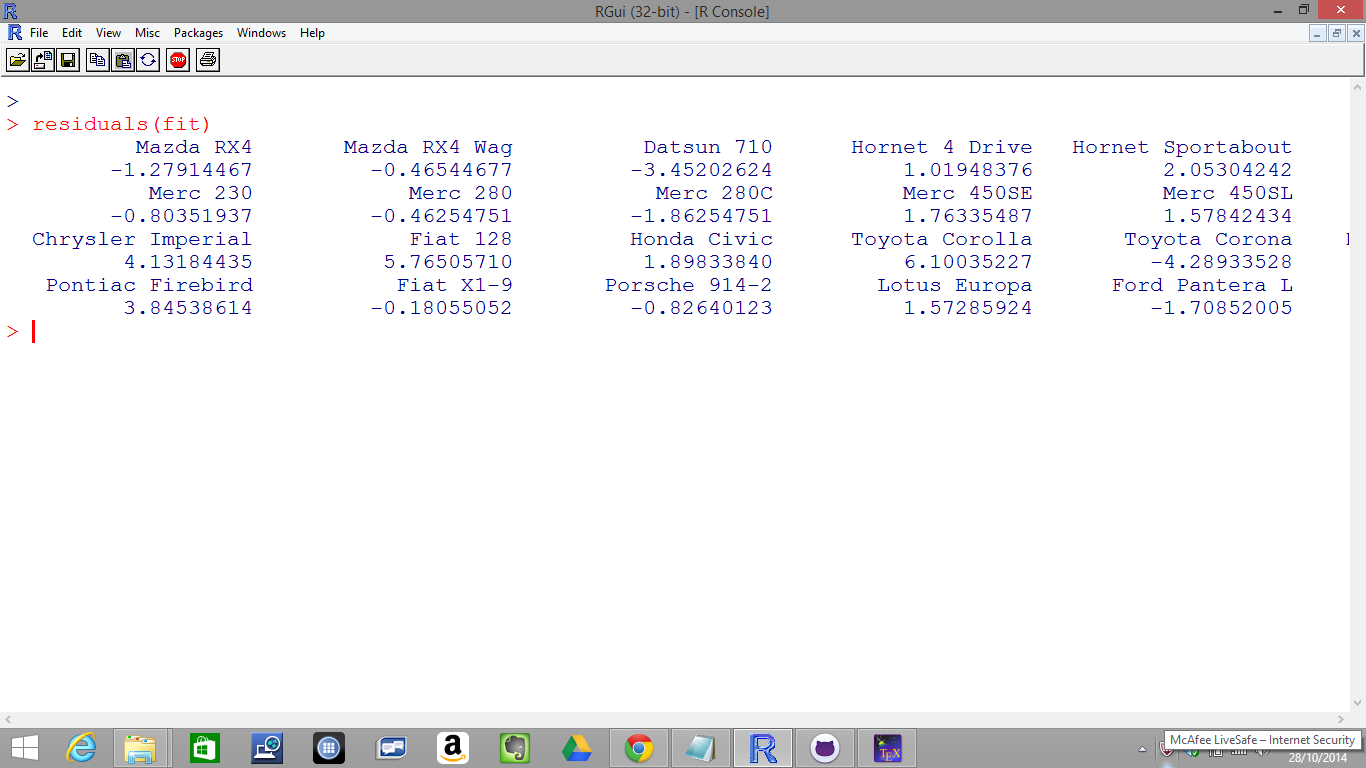
\includegraphics[width=0.9\linewidth]{screenshot1}
\caption{}
\label{fig:screenshot1}
\end{figure}
\begin{verbatim}
> sum(residuals(fit))
[1] 1.096345e-15

> #Shapiro-Wilk Test for Normality
> shapiro.test(resid(fit))
 
 Shapiro-Wilk normality test
 
 data:  resid(fit)
 W = 0.9375, p-value = 0.06341
 
 
\end{verbatim}

\newpage
\subsubsection*{Weighted Residuals}
\begin{framed}
\begin{verbatim}
x <- 1:10
w <- 0:9
y <- rnorm(x)
weighted.residuals(lmxy <- lm(y ~ x, weights = w))
\end{verbatim}
\end{framed}

\end{document}
